% !TEX encoding = UTF-8 Unicode
\documentclass{report}
%\usepackage{xeCJK}

%\setCJKmainfont{微软雅黑}
\title{Mini Project Report}
\author{Li Chen}
\date{\today}
	
% big font for sections
\usepackage{sectsty}
\usepackage{setspace}
\sectionfont{\LARGE}

\usepackage{graphicx}
\usepackage{wrapfig}
\usepackage{caption}
\usepackage{subcaption}
\usepackage{listings}
\usepackage{array}
\usepackage{titlesec}
\setcounter{secnumdepth}{5}
\usepackage[colorlinks,
linkcolor=black,
anchorcolor=black,
citecolor=black
]{hyperref}
\lstset{
    columns=fixed,       
    numbers=left,                                        % 在左侧显示行号
    frame=none,                                          % 不显示背景边框
    backgroundcolor=\color[RGB]{245,245,244},            % 设定背景颜色
    keywordstyle=\color[RGB]{40,40,255},                 % 设定关键字颜色
    numberstyle=\footnotesize\color[RGB]{0,0,0},           % 设定行号格式
    commentstyle=\it\color[RGB]{0,96,96},                % 设置代码注释的格式
    stringstyle=\rmfamily\slshape\color[RGB]{128,0,0},   % 设置字符串格式
    showstringspaces=false,                              % 不显示字符串中的空格
    language=c,                                        % 设置语言
    morekeywords={alignas,continute,friend,register,true,alignof,decltype,goto,
    reinterpret_cast,try,asm,defult,if,return,typedef,auto,delete,inline,short,
    typeid,bool,do,int,signed,typename,break,double,long,sizeof,union,case,
    dynamic_cast,mutable,static,unsigned,catch,else,namespace,static_assert,using,
    char,enum,new,static_cast,virtual,char16_t,char32_t,explict,noexcept,struct,
    void,export,nullptr,switch,volatile,class,extern,operator,template,wchar_t,
    const,false,private,this,while,constexpr,float,protected,thread_local,
    const_cast,for,public,throw,std, CHECK_THROW, CHECK_EQUAL, vector},
}

% \begin{comment} ... \end{comment{}
%\usepackage{verbatim}

\setlength{\parskip}{0pt}

\makeatletter
\renewcommand{\paragraph}{
  \@startsection{paragraph}{4}
    {\z@}{1.25ex \@plus 1ex \@minus .2ex}{-1em}
      {\normalfont\normalsize\bfseries}
      }
      \makeatother

\usepackage[
	sorting=none,
	minbibnames=8,
	maxbibnames=9,
	block=space,
	backend=biber
]{biblatex}
\bibliography{publications}


\usepackage{parskip}

\usepackage{lipsum}

\begin{document}

\newpage

\maketitle

\newpage

\renewcommand{\contentsname}{Table of Content}
\tableofcontents


%=================
\begin{spacing}{1.5}
\section{introduction}
	\subsection{Overview}
	A "binary bomb" is a program provided to students as an object code file. When run, it prompts the user to type in 6 different strings. If any of these is incorrect, the bomb ``explodes,'' printing an error message and logging the event on a grading server. Students must ``defuse'' their own unique bomb by disassembling and reverse engineering the program to determine what the 6 strings should be. The lab teaches students to understand assembly language, and also forces them to learn how to use a debugger. It's also great fun. A legendary lab among the CMU undergrads.
	\subsection{Preparation}
	在拆除炸弹之前,首先进行一些前期准备:
	\begin{itemize}
		\item	通过putty登陆服务器,发现我本次Lab的实验文件:\textbf{bomb51.tar}
		\item	执行\textbf{tar xvf bomb51.tar}解压文件,得到四个文件:bomb bomb.c ID README
		\item	其中 ID README 分别是学生的编号和这次的说明文档。
		
				于是查看\textbf{bomb.c}, 发现其头文件声明如下:
				\lstinputlisting{sources/header.txt}
				
				phase.h包含了这次炸弹的全部关卡,而它并没有在Lab中给出。因此我们只能从可执行文件\textbf{bomb}下手
		\item	执行\textbf{objdump -d bomb > bomb.txt}, 反编译可执行文件,将汇编代码输出到\textbf{bomb.txt}
		\item	反编译之后的代码非常长,不过在仔细研究之后,发现其中有六个函数\textbf{<phase$\_$1..6>},分别对应六个关卡。因此,这次Lab的关键就是破解这六个关卡对应的汇编代码,分析这六个函数的功能。
	\end{itemize}
\section{phase$\_$1}
	第一关的汇编代码如下:
	\begin{figure}[h]
		\centering
			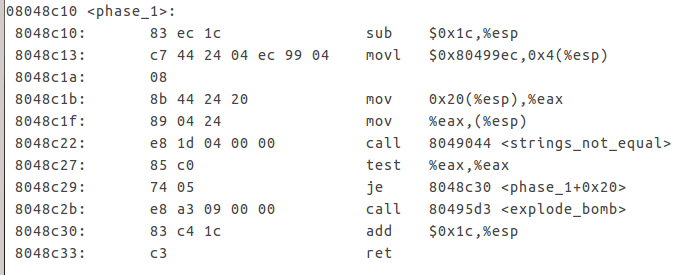
\includegraphics[scale=0.77]{images/phase_1.png}
	\end{figure}
	这个函数较短,分析发现,它调用了一个名为\textbf{strings$\_$not$\_$equal}函数。
	
	分析\textbf{strings$\_$not$\_$equal}这个函数,发现它实现这样一个功能:比较两个字符串,相等返回0,不相等返回1
	
	分析call之后的程序,发现如果返回值(即$\%eax$)不为0的话,会调用\textbf{explode$\_$bomb}函数,炸弹会被引爆。因此,我们输入的字符串应该与某个字符串相同。
	
	这样,破解phase$\_$1的方法就很清晰了:

		\begin{center}
			\textbf{输入存在地址0x80499ec中的字符串}
		\end{center}

	于是现在的问题是找出存放在地址0x80499ec中的字符串。
	
	从调用strings$\_$not$\_$equal的语句向上看:
	\begin{figure}[h]
		\centering
			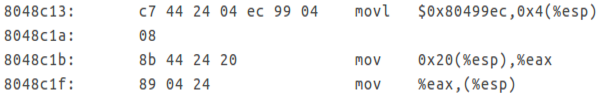
\includegraphics[scale=0.77]{images/phase_1_part_0.png}	
	\end{figure}
	
	这表示,这个函数的两个参数,一个是程序自身地址\textbf{0x80499ec},另一个\textbf{0x20(\%esp)}就是我们的输入参数。
	
	我们首先需要知道\textbf{0x80499ec}地址里存放的数据。于是使用\textbf{gdb},输入命令\textbf{p (char *) 0x80499ec},查看它存放的数据:
	\begin{figure}[h]
		\centering
			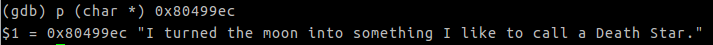
\includegraphics[scale=0.7]{images/phase_1_part_1.png};
	\end{figure}
	
	第一关的答案水落石出:输入\textbf{I turned the moon into something I like to call a Death Star.},顺利过关。
	
	主要复习知识点:\textbf{常量的存储、函数的参数传递}
	
\section{phase$\_$2}
	\begin{itemize}
	\item
	第二关的汇编代码如下:
	\begin{figure}[h]
		\centering
			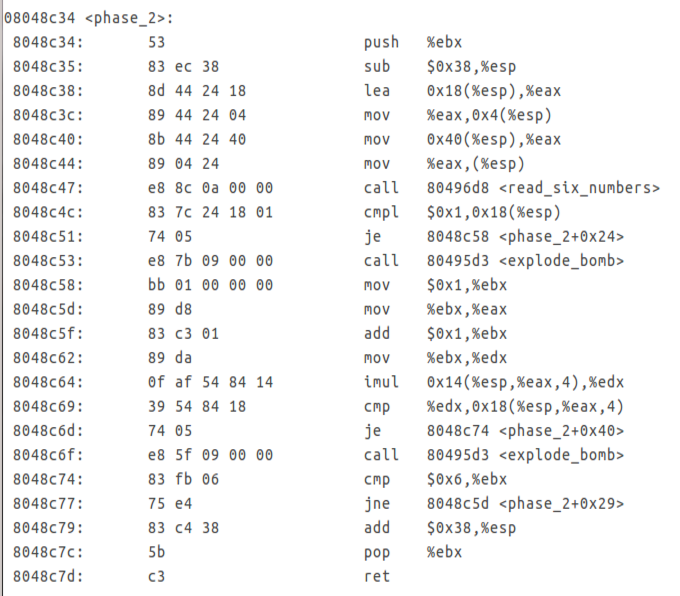
\includegraphics[scale=0.77]{images/phase_2.png}
	\end{figure}
	
	\item
	我们首先发现,它调用了一个\textbf{read$\_$six$\_$numbers}函数。经过分析,这个函数从输入中读入六个整数,并按地址从低到高存放在\textbf{0x18($\%$esp) - (0x30$\%$esp)}这24个字节中。也就是说,\textbf{a[0]}在\textbf{0x18($\%$esp)},\textbf{a[1]}在\textbf{0x1c($\%$esp)},以此类推。
	
	\item
	然后观察下面一段代码:
	
	\begin{figure}[h]
		\centering
			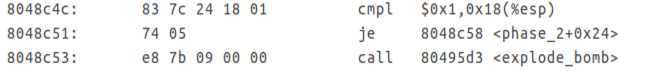
\includegraphics[scale=0.77]{images/phase_2_part_0.png}
	\end{figure}
	
	\item
	这段代码将\textbf{0x18($\%$esp)}即\textbf{a[0]}与$1$进行比较,如果不等则炸弹爆炸。这一段说明,我们输入的第一个数必须为1。
	
	\item
	接下来是一个循环:

	\begin{figure}[h]
		\centering
			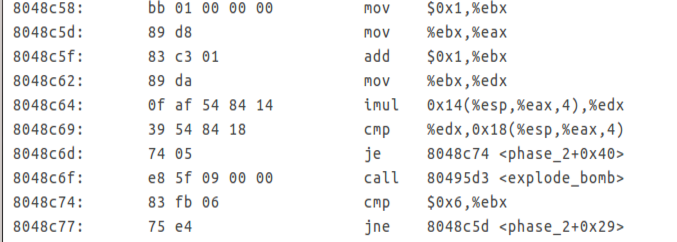
\includegraphics[scale=0.77]{images/phase_2_part_1.png}
	\end{figure}
		
	这个循环的循环变量是\textbf{$\%$ebx},从2循环到 5。同时, \textbf{$\%$eax}始终为
\textbf{$\%$ebx - 1}
	中间的判断语句,可以发现它是将\textbf{0x14($\%$esp, $\%$eax, 4) * $\%$edx}相乘,并与\textbf{0x18($\%$esp, $\%$eax, 4)}比较。由于a数组的起始位置为\textbf{0x18($\%$esp)}, 这两个地址就是\textbf{a[$\_$eax - 1]}和\textbf{a[$\_$eax]}。

	因此,其对应的c语言代码如下:

	\lstinputlisting{sources/phase_2.txt}
	
	\item
	这个函数表明,我们输入的数组a要满足以下条件:
	\begin{itemize}
		\item	数组长度为6
		\item	a[0] = 1
		\item	a[i] = a[i - 1] * (i + 1)
	\end{itemize}

	\item
	所以,第二关的答案就水落石出了: \textbf{1 2 6 24 120 720}
	
	\end{itemize}
	
	\begin{figure}[h]
		\centering
			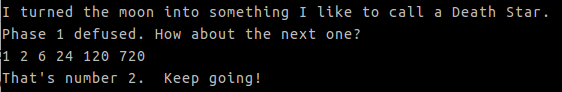
\includegraphics[scale=0.8]{images/phase_2_success.png};
	\end{figure}
	考察知识点:数组的存储	
\section{phase$\_$3}
	\begin{itemize}
	\item
	第三关的汇编代码如下:
	\begin{figure}[h]
		\centering
			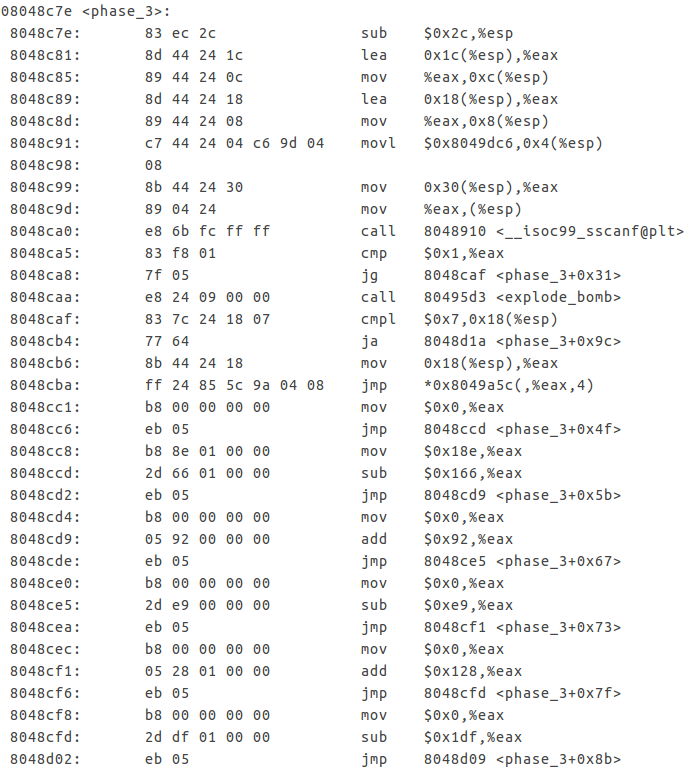
\includegraphics[scale=0.73]{images/phase_3.png}
	\end{figure}
	
	\newpage

	\begin{figure}[h]
		\centering
			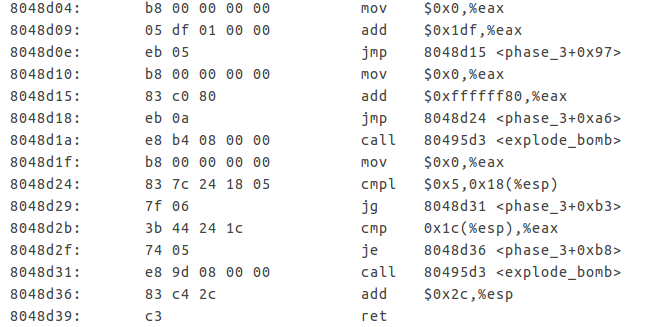
\includegraphics[scale=0.73]{images/phase_3_1.png}
	\end{figure}
	
	\item
	首先看到它调用了\textbf{sscanf}函数,参数存放在\textbf{0x8049dc6}地址中。
	
	于是首先用gdb查看\textbf{0x8049dc6}地址中的参数:

	\begin{figure}[h]
		\centering
			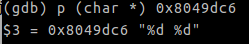
\includegraphics[scale=0.8]{images/phase_3_part_0.png}
	\end{figure}	
	
	“$\%d \%d$”代表读入了两个整数。调用sscanf结束后,将sscanf的返回值与1比较,若不大于1则炸弹爆炸。
	
	由此可以得到我们这关的目标是输入两个整数\textbf{a b}。
	
	\item
	输入的两个整数\textbf{a b}存放在\textbf{0x18($\%$esp)} 和 \textbf{0x1c($\%$esp)}中。接着往下看程序:
		
		
	\begin{figure}[h]
		\centering
			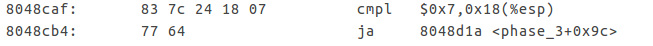
\includegraphics[scale=0.77]{images/phase_3_part_1.png}
	\end{figure}

	这里可以发现,程序将\textbf{0x18($\%$esp)}, 即输入的第一个整数\textbf{a}与7进行比较,如果大于7则炸弹爆炸。同时,由于使用的是\textbf{ja}命令,即\textbf{a}为无符号数,\textbf{a}应该不小于0
	
	这样我们可以得出第一个限制条件:输入的第一个	整数 $0 \le a \le 7$
	
	继续往下看,注意到这一段:	
	\begin{figure}[H]
		\centering
			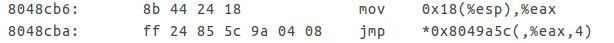
\includegraphics[scale=0.77]{images/phase_3_part_2.png}
	\end{figure}

	\item
	这段具有很明显的\textbf{switch}语句的特征,而跳转表存放在\textbf{0x8049a5c}中。
\newpage		
	于是调用gdb,先查看对应的跳转表:	
	\begin{figure}[h]
		\centering
			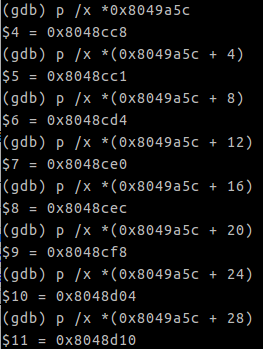
\includegraphics[scale=0.77]{images/phase_3_part_3.png}
	\end{figure}
	
	这样可以将接下来的代码划分模块:	
	
	\begin{figure}[h]
		\centering
			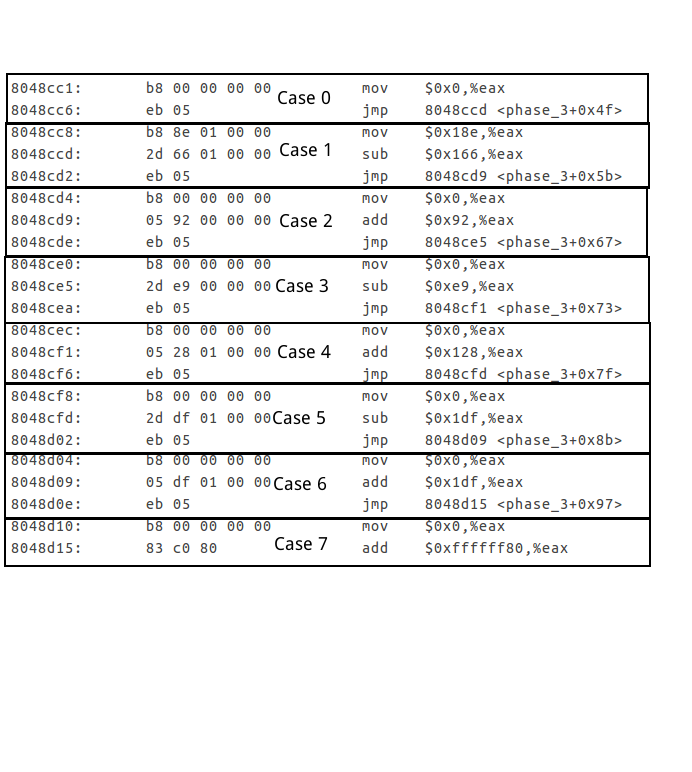
\includegraphics[scale=0.77]{images/phase_3_part_4.png}
	\end{figure}
	
	\item
	于是可以得出对应的c语言代码:
	
	\lstinputlisting{sources/switch_origin.txt}

	经过整理后的代码如下:
	
	\lstinputlisting{sources/switch.txt}
	
	\item
	在switch语句段后,有这么一段:
	
	\begin{figure}[h]
		\centering
			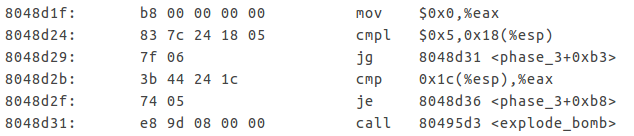
\includegraphics[scale=0.77]{images/phase_3_part_5.png}
	\end{figure}
	
	这里给出了第二个限制条件: 输入的第一个整数$a \le 5$
	
	最后,程序将输入的第二个整数\textbf{b}与switch的结果进行比较,不同则炸弹爆炸。
	
	\item
	因此,这关的答案就水落石出了:
		\begin{center}
			输入一个整数$a(0 \le a \le 5)$, 和a经过switch之后的结果b
		\end{center}
	\end{itemize}		
	选用\textbf{a = 4, b = 168},顺利过关

\section{phase$\_$4}
	第四关的汇编代码如下:
	\begin{figure}[h]
		\centering
			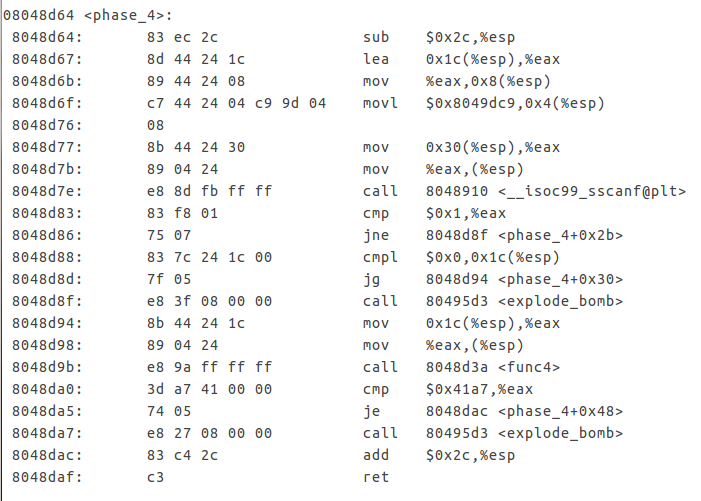
\includegraphics[scale=0.77]{images/phase_4.png}
	\end{figure}
	
	首先,它和phase$\_$3一样,调用了sscanf函数。和上一个函数的处理方法一样,运用gdb,发现sscanf的参数是\textbf{"$\%$d“},即读入一个整数n,存放在\textbf{0x1c($\%$esp)}。
	
	读入后,将n与0比较,如果$n \le 0$炸弹就会爆炸。
	
	因此,我们得到了第一个限制条件: $n > 0$
	
	随后,将n作为参数传入函数\textbf{func4}中。
	
	%一段代码
	
	这段代码表示,如果函数的返回值不为\textbf{0x41a7},则炸弹爆炸。
	
	这样就知道了第四关的要求:找出使\textbf{func4}的结果为\textbf{0x41a7}的输入值。
	
	于是我们开始研究\textbf{func4}函数。
	
	\begin{figure}[h]
		\centering
			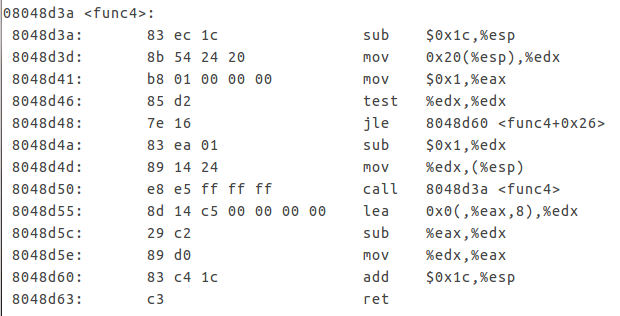
\includegraphics[scale=0.77]{images/fun_4.png}
	\end{figure}
	
	分析这一个函数,可以得出它的作用如下:
	
	\begin{itemize}
		\item	首先,函数将返回值置为1。
		\item	如果传入参数$x \le 0$,则直接返回。
		\item	递归调用\textbf{fun4}
		\item	将递归的结果乘7后作为返回值
	\end{itemize}
	
	对应的C语言代码如下:
	\lstinputlisting{sources/fun4.txt}
	
	因此,我们的问题变成:$\log_7(0x41a7)$ = ?
	
	经过计算得出,$7 ^ 5 = 16807 = 0x41a7$
	
	输入5,成功过关。
\section{phase$\_$5}

	\begin{itemize}

	\item
	
	第五关的汇编代码如下:
		
	\lstinputlisting[language={[x86masm]Assembler}]{sources/phase_5.asm}
	
	\item
		
	\lstinputlisting[language={[x86masm]Assembler}]{sources/phase_5_part_1.asm}
	
	首先,我们发现它调用了\textbf{string$\_$length}这个函数,并且将返回值与$6$进行比较,不相等的话炸弹会爆炸。查看\textbf{string$\_$length}的代码发现,它的功能为返回一个字符串的长度。
	
	因此,我们得到了第一个限制条件:需要输入一个长度为6的字符串。

	\item
		
	\lstinputlisting[language={[x86masm]Assembler}]{sources/phase_5_part_2.asm}
	
	这里是一个循环,循环变量是$\%eax$,范围从0到5。

	\item
	
	\lstinputlisting[language={[x86masm]Assembler}]{sources/phase_5_part_3.asm}
	
	\textbf{movsbl}这个语句的意思为,将位于$Mem[\%ebx + \%eax]$处地址的数据最低位取出,进行符号位扩展后送入$\%edx$中,结合后面一句\textbf{and  $\$0xf, \%edx$},以及$\%$ebx即为输入字符串的首地址,可以发现这句话的意思是取出输入字符串第\textbf{$\%$eax}位ASCII码的后四位。	
	
	\item
	\lstinputlisting[language={[x86masm]Assembler}]{sources/phase_5_part_4.asm}
	
		
	这个语句将刚刚取出的值作为下标,在从\textbf{0x8049a7c}开始的数组中进行寻值,并将结果构成新的字符串压入栈中。于是,我们调用gdb命令,查看\textbf{0x8049a7c}地址对应的值。
	
	\begin{figure}[h]
		\centering
			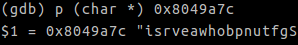
\includegraphics[scale=0.8]{images/phase_5_part_5.png}
	\end{figure}	
	
	这里相当于是一个密码加密的过程,即将每一个原先的字母用一个一一对应的字母替换。

	\item
		
	\lstinputlisting[language={[x86masm]Assembler}]{sources/phase_5_part_6.asm}
	
	这里又向栈中压入了一个\textbf{0x8049a52}地址中的数据,并且调用\textbf{strings$\_$not$\_$equal}函数。根据之前的分析,如果传入的两个字符串不等,炸弹就会爆炸。因此,我们生成的字符串应该与\textbf{0x8049a52}地址中的相同。
	
	\item
	
	于是调用gdb,查看\textbf{0x8049a52}地址中的内容:
	\begin{figure}[h]
		\centering
			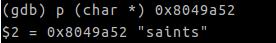
\includegraphics[scale=0.8]{images/phase_5_part_7.png}
	\end{figure}	
		
	\item
		
	因此,我们只需要生成“saints”这个字符串即可。根据索引表,“saints”这六个字母对应的索引值分别为1, 5, 0, 11, 13, 1。
	
	我们只需要输入六个ASCII码低4位为这六个值的字符即可。于是选用 \textbf{a, e, 0, k, m, a}。
	
	\end{itemize}
	
	输入\textbf{ae0kma},顺利过关。
	
	\begin{figure}[h]
		\centering
			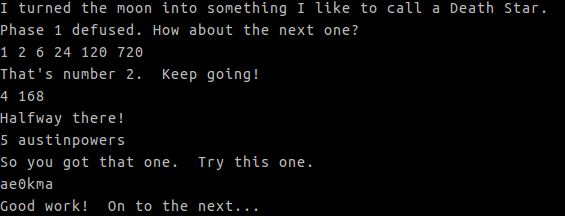
\includegraphics[scale=0.8]{images/phase_5_success.png}
	\end{figure}	
\section{phase$\_$6}

	\begin{itemize}
	
	\item
	
	第六关的汇编代码如下:
		
	\lstinputlisting[language={[x86masm]Assembler}]{sources/phase_6.asm}

	\item
	
	首先发现它调用了\textbf{strtol}这个函数。观察这个函数的代码发现,它需要传入三个参数,这里分别为\textbf{$\%eax$, 0 和 0xa}。\textbf{strtol}的主要功能可以用以下c语言代码表示:

	\lstinputlisting{sources/strtol.txt}	
	
	这段代码的作用就是将输入的字符串转换为对应的base进制数表示。

	\item
	
	\lstinputlisting[language={[x86masm]Assembler}]{sources/phase_6_part_1.asm}
	
	这里调用了函数\textbf{fun6}。由于传入的是一个地址\textbf{0x804c174},因此fun6的返回值是固定的,因此,经过一系列跳转后,在\textbf{cmp $\%$edx, ($\%$eax)}中, ($\%$eax)的值也是一定的。运用gdb设置断点,查看得知此时($\%$eax)的值为268。

	\item	

	由于$\%$edx的值就是我们输入的字符串,答案就唾手可得了。
	
	\end{itemize}
	
	输入\textbf{268},顺利过关。
	
	\begin{figure}[h]
		\centering
			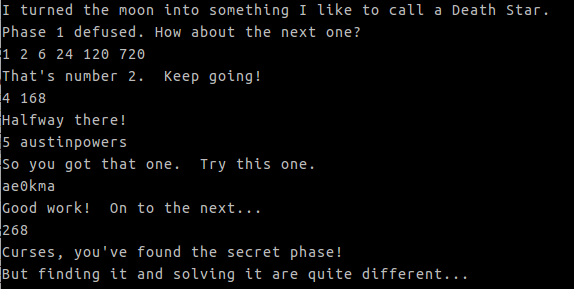
\includegraphics[scale=0.77]{images/phase_6_success.png}
	\end{figure}	

\section{secret$\_$phase}

\section{conclusion}

	这次的Bomb Lab总计花了我7个小时,从晚上6点拆到凌晨1点,才算大功告成。不可否认,这个lab对我对于汇编的理解起到了很强的巩固作用。从一开始面对冗长汇编代码的手足无措,到一步步将炸弹抽丝剥茧,慢慢拆弹,到最后将隐藏关解决,这其中的每一关对我都是新的挑战。
	
	这次lab的覆盖范围非常广泛:第一关的函数调用,第二关的数组的存储,第三关的switch跳转表的实现。。几乎每一关的知识点都不重合,设计者的用心良苦可见一斑。
	
	同时,通过这次lab, 我也系统学习了gdb的使用。在平常的编程环境中,我们常常只需要在IDE中用鼠标设置断点,点开watch窗口,就可以轻松享用IDE的调试功能,却很少想过这些调试功能都是怎么实现的。通过这次一步步的手动输入gdb命令,我对于IDE的调试功能有了一个粗浅的了解。当然,对于主流IDE调试功能的更深层次的实现,是我接下来需要探索的。
	
	陆游说过:“纸上得来终觉浅,绝知此事要躬行。” 对于CSAPP这门课来说,更是如此。通过这次lab,通过大量的读代码,gdb调试,我对于代码的底层实现有了新的认识。我想,这就是老师布置这次lab的用意之一吧。

\end{spacing}

%=================

\end{document}
